%%%
%% This is file `sample-sigplan.tex',
%% generated with the docstrip utility.
%%
%% The original source files were:
%%
%% samples.dtx  (with options: `sigplan')
%%
%% IMPORTANT NOTICE:
%%
%% For the copyright see the source file.
%%
%% Any modified versions of this file must be renamed
%% with new filenames distinct from sample-sigplan.tex.
%%
%% For distribution of the original source see the terms
%% for copying and modification in the file samples.dtx.
%%
%% This generated file may be distributed as long as the
%% original source files, as listed above, are part of the
%% same distribution. (The sources need not necessarily be
%% in the same archive or directory.)
%%
%%
%% Commands for TeXCount
%TC:macro \cite [option:text,text]
%TC:macro \citep [option:text,text]
%TC:macro \citet [option:text,text]
%TC:envir table 0 1
%TC:envir table* 0 1
%TC:envir tabular [ignore] word
%TC:envir displaymath 0 word
%TC:envir math 0 word
%TC:envir comment 0 0
%%
%%
%% The first command in your LaTeX source must be the \documentclass command.
%%\documentclass[sigplan,nonacm]{acmart}
\documentclass[sigplan, nonacm]{acmart}\settopmatter{printfolios=true,printccs=false,printacmref=false}

\graphicspath{{pictures/}}
%%
%% \BibTeX command to typeset BibTeX logo in the docs
\AtBeginDocument{%
	\providecommand\BibTeX{{%
			\normalfont B\kern-0.5em{\scshape i\kern-0.25em b}\kern-0.8em\TeX}}}

%% Rights management information.  This information is sent to you
%% when you complete the rights form.  These commands have SAMPLE
%% values in them; it is your responsibility as an author to replace
%% the commands and values with those provided to you when you
%% complete the rights form.
%%\setcopyright{acmcopyright}
\setcopyright{none}
%%\acmJournal{PACMPL}
%%\acmVolume{1}
%%\acmNumber{CONF} % CONF = POPL or ICFP or OOPSLA
%%\acmArticle{1}
%%\acmYear{2021}
%%\acmMonth{9}
%%\acmDOI{}
%%\copyrightyear{2018}
%%\acmYear{2018}
%%\acmDOI{10.1145/1122445.1122456}

%% These commands are for a PROCEEDINGS abstract or paper.
%%\acmConference[Woodstock '18]{Woodstock '18: ACM Symposium%% on Neural
%%  Gaze Detection}{June 03--05, 2018}{Woodstock, NY}
%%\acmBooktitle{Woodstock '18: ACM Symposium on Neural Gaze Detection,
%%  June 03--05, 2018, Woodstock, NY}
%%\acmPrice{15.00}
%%\acmISBN{978-1-4503-XXXX-X/18/06}


%%
%% Submission ID.
%% Use this when submitting an article to a sponsored event. You'll
%% receive a unique submission ID from the organizers
%% of the event, and this ID should be used as the parameter to this command.
%%\acmSubmissionID{123-A56-BU3}

%%
%% The majority of ACM publications use numbered citations and
%% references.  The command \citestyle{authoryear} switches to the
%% "author year" style.
%%
%% If you are preparing content for an event
%% sponsored by ACM SIGGRAPH, you must use the "author year" style of
%% citations and references.
%% Uncommenting
%% the next command will enable that style.
%%\citestyle{acmauthoryear}

%%
%% end of the preamble, start of the body of the document source.
\begin{document}
\sloppy

%%
%% The "title" command has an optional parameter,
%% allowing the author to define a "short title" to be used in page headers.
\title{Parallel training by Pipeline Execution In AIRCoP}

%%
%% The "author" command and its associated commands are used to define
%% the authors and their affiliations.
%% Of note is the shared affiliation of the first two authors, and the
%% "authornote" and "authornotemark" commands
%% used to denote shared contribution to the research.
\author{Ruiqi Gao}
\email{gao606@purdue.edu}
\affiliation{%
  \institution{Purdue University}
  \city{Lafayette}
  \state{Indiana}
  \country{USA}
  \postcode{47901}
}

\begin{abstract}
  Various approaches like data parallelism, model parallelism, attribute parallelism, and pipeline parallelism have been developed to train machine learning models in parallel. However, no existing frameworks have integrated these approaches successfully. Most generally used machine learning frameworks such as TensorFlow and Pytorch only support a tiny subset of parallel paradigms, i.e., data parallelism and model parallelism. GPipe and PipeDream support different types of pipeline parallelism by dividing the model into several modules and running them in a pipeline fashion.
  AIRCop (Abstract IR for Comprehensive Parallelization) is a developing project that unifies all the parallelism paradigms mentioned above. Since all the machine learning models can be viewed as computation graphs, parallelism paradigms are just different kinds of computation graph transformation, i.e., transformation pass. AIRCop uses this idea, takes a machine learning model and parallelization annotations that describe the desired parallel behavior as input, and generates target program through different transformation passes.

\end{abstract}

\keywords{Parallel Training, Graph Transformation, Machine Learning Frameworks, Pipeline Parallelism}

\maketitle
\section{Proposal Retrospect and Progress}
\subsection{Proposal Retrospect}
The proposal mentions that this project will support both stacked pipeline and queued pipeline. However, we currently only support stacked pipeline for pipeline execution. The reason is that we spend some time adding support for multiple-module for AIRCoP because AIRCoP initially only support single module. This work involves changing the syntax of the frontend to make writing multiple-module models intuitive and easy. After finishing support for the stacked pipeline, we also find that the Memory Management problem in AIRCoP will cause a significant performance overhead. AIRCoP initially uses cudaMalloc and cudaFree inside the training loop for memory allocation. Due to the complex synchronization mechanism of cudaMalloc/Free, these operations will occupy a very long time. After analyzing the running time with NVIDIA profiler, we find that most of the execution time is spent on cudaMalloc/Free. It is even 10x faster by pre-allocating the memory before the training loop, so we focus on addressing the memory management problem after finishing stacked pipeline. We use code-motion techniques to lift all the cudaMalloc out of the training loop for optimization.\par
 Queued pipeline parallelism performs asynchronous weight updates and uses lagged network weight, so we choose to address the memory management problem first due to limited time.\par
All the pipeline parallelism used in this paper refers to stacked pipeline parallelism because we currently only implement stacked pipeline.
\subsection{Progress}
Although we only support stacked pipeline, it is sufficient for multi-module pipeline parallelism. We can still mix spatial partition with pipeline execution to explore different parallelism settings and gain insight into parallel training, which we will present in the evaluation.\par
Our progress is shown as follows:
\begin{itemize}
  \item We formalize the transformation procedure of stacked pipeline as training loop transformation on the formal language of AIRCoP.
  \item We implement stacked pipeline for AIRCoP.
  \item We optimize the memory management for AIRCoP.
  \item We run evaluation benchmarks with different parallelism settings (Spatial Partition, Spatial Partition mixed with Pipeline Execution) to validate our implementation and gain some insight into parallel training.
\end{itemize}
The paper is organized as follows: \par \par
In section \ref{introduction}, we introduce parallel training, different existing parallelism strategies, and AIRCoP.\par
In section \ref{pipelineparallism}, we further study stacked pipeline - the pipeline parallelism we support in AIRCoP.\par
In section \ref{formalpipe}, we demonstrate the formal description of the training loop transformation for pipeline parallelism.\par
In section \ref{implementation}, we present the implementation detail of our work.\par
In section \ref{evaluation}, we offer a parallel training evaluation with different parallelism settings to illustrate the flexibility of our framework.\par
In section \ref{conclusion}, we summarize our progress and draw some conclusions.
\section{Introduction} \label{introduction}
Real-world machine learning applications are usually enormous. They require excessive data for training and cannot work on a single device. Therefore, various parallel strategies have been proposed for running large models in parallel among multiple distributed devices to achieve optimal performance.\par
 \subsection{Spatial Partition}
 The most common strategy for parallel training is Spatial Partition, where the data/weight/operation is partitioned across multiple devices. Among different Spatial Partition parallelism strategies, Data Parallelism\cite{krizhevsky2012imagenet}, where we split input across multiple devices and maintain the same network weight, is the simplest one. Data Parallelism is adapted and developed by most modern machine learning frameworks, e.g., TensorFlow\cite{abadi2016tensorflow} and Pytorch\cite{paszke2019pytorch}. Data Parallelism requires network weight synchronizations amid devices at the end of each iteration. Therefore, Data Parallelism is ideal for a computation-intensive network with few weight parameters, e.g., convolution and pooling layer, but will introduce significant communication overhead for a network with heavy weight parameters like fully-connected layers.\par
  Model parallelism\cite{dean2012large} is another Spatial Partition based parallelism strategy and is achieved by splitting the network weight tensor across devices while broadcasting the input tensor. Model parallelism reduces the communication overhead of Data Parallelism but is rarely used because dependencies often exist between network layers. Attribute parallelism\cite{jia2019beyond} can partition the attribute dimension in both input and weight parameters and require collective communication like AllReduce between operations. An experienced developer can combine different Parallelism strategies to achieve optimal performance, e.g., a previous work\cite{krizhevsky2014one} uses data parallelism for the convolution layer and model parallelism for the fully-connected layer.\par
 \subsection{Pipeline Parallelism}
 Unlike Spatial Partition, where input data/weight is distributed across multiple devices, Pipeline Parallelism splits a machine learning model into several modules with data dependency between them while dividing a batch into several micro-batches. It then runs different modules in parallel in a pipelined fashion. Both GPipe\cite{huang2019gpipe} and Pipedream\cite{narayanan2019pipedream} study and develop Pipeline Parallelism. Pipeline Parallelism is especially useful when the training system has low-bandwidth connections because it can limit the communication overhead to only happen at module boundaries.\par
 As shown in \cite{krizhevsky2014one}, combining different parallelism strategies can achieve better performance for different applications. However, no existing machine learning framework can support all the parallelism strategies. TensorFlow\cite{abadi2016tensorflow} and Pytorch\cite{paszke2019pytorch} only support Data Parallelism while GPipe\cite{huang2019gpipe} and Pipedream\cite{narayanan2019pipedream} only implement Pipeline Parallelism. Users are limited to a subset of Parallelism strategies and cannot fully utilize the distributed training system.\par
  Different distributed system topologies also would require different strategies for optimal performance. As we mentioned before, Spatial Partition may introduce frequent tensor communication overhead between operations.
 \begin{figure}[htbp]
  \centering
  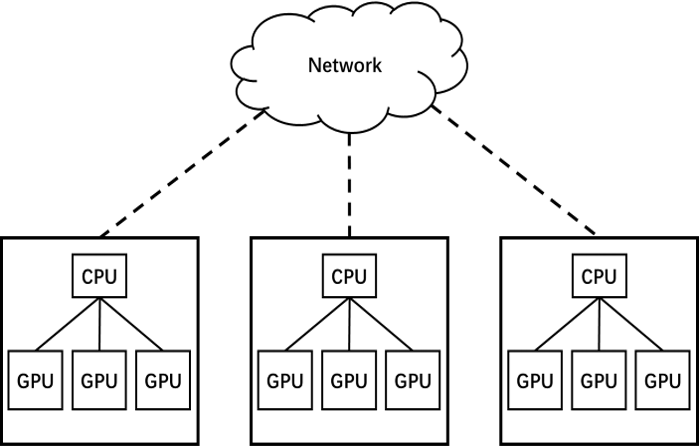
\includegraphics[scale=0.7]{networktopo.png}
  \caption{Large training system}
  \label{fig:networktopo}
\end{figure} This overhead may be negligible for a GPU Cluster with high-bandwidth interconnections but will cause a significant performance drop for large distributed systems consisting of several GPU clusters with low bandwidth connections among them as shown in Figure \ref{fig:networktopo}. Large training servers are often deployed across multiple nodes because high bandwidth inter-GPU connection techniques like NV-Link can only scale to a limited number of devices. It will be ideal if we can divide the model into several modules, assign each module to a cluster, use Spatial Partition inside a GPU cluster, and adopt Pipeline Parallelism among modules.\par
\subsection{AIRCoP}
AIRCoP \cite{aircopfeiwang} is a machine learning framework that supports all the parallel parallelisms above, thus allowing users to explore different parallel settings. AIRCoP has previously implemented Spatial Partition, and our work implements Pipeline Parallelism for AIRCoP, thus making AIRCoP a unifying parallel training framework.\par
 %\begin{figure}[htbp]
 % \centering
 % 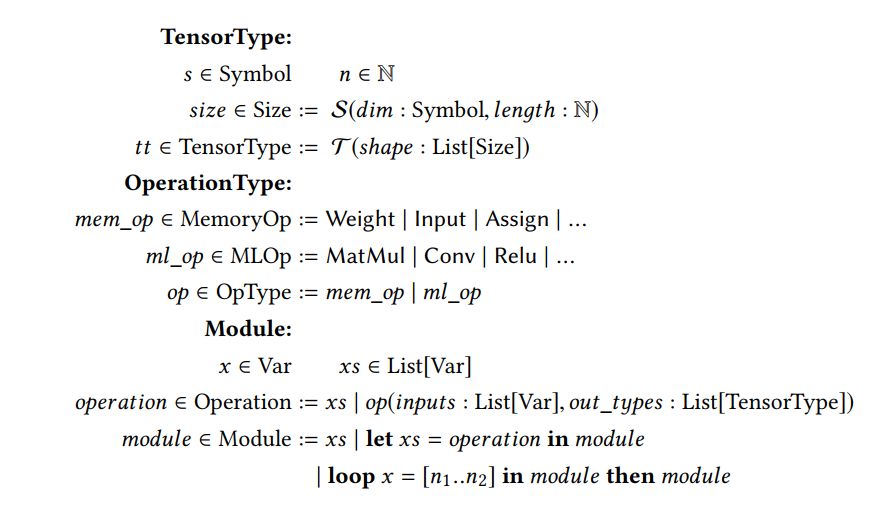
\includegraphics[scale=0.7]{FormalSyntax}
 % \caption{Formal Syntax of AIRCoP}
 % \label{fig:sample}
%\end{figure}
\begin{align*}\label{formalsyntax}
  \textbf{TensorType}:& \\
  s \in Symbol& \quad n  \in \mathbb{N} \\
  size \in Size& :=\mathcal{S}(dim:Symbol,length:\mathbb{N})\\
  tt\in TensorType& := \mathcal{T}(shape:List[Size])\\
  \textbf{OperationType}:& \\
  mem\_op\in MemoryOp& := Weight \text{ } | \text{ } Input \text{ } | \text{ } Zero \text{ } | \text{ } One \text{ } \dots \\
  ml\_op \in MLOP& := MatMul \text{ } | \text{ } Conv \text{ } | \text{ } AvgPool \text{ }\text{ } | \dots \\
  op \in OperationType&:= mem\_op \text{ } | \text{ } ml\_op \\
\end{align*}
\begin{align*}
  \textbf{Module}:& \\
  x \in Var& \quad \quad \quad xs \in List[Var]\\
  operation \in Operation&:= xs \text{ } | \text{ } op(inputs: List[Var], \\
  & out\_types:List[TensorType]) \\
  module \in Module&:=xs \text{ } | \text{ } \textbf{let } xs=operation \textbf{ in } module \\
  \textbf{Model}:&\\
  model \in Model&:= \quad List[Module]
\end{align*}
AIRCoP develops a formal syntax to represent tensor computation graphs. The syntax mainly has three components: 1. Tensor and corresponding TensorType to represent input tensor and weight. 2. Operation and corresponding Operation Type to represent different Machine learning operations like Conv/MatMul/Relu and their input/output Type. 3. Module to represent different modules.\par
Operations are connected through let-bindings. Furthermore, we use annotation of the formal syntax to represent different parallelism strategies. We develop annotation systems for both Tensor, Operation, and Module. Tensor and Operation annotation represents Spatial Partition by indicating the dimension to partition, and Module annotation represents the number of micro-batches. Users only need to write the sequential forward computation of the Machine Learning model, and the correct final training loop will be automatically computed through a series of transformations.
 \section{Pipeline Parallelism} \label{pipelineparallism}
 Pipeline Parallelism is ideal for distributed training among several nodes with weak inter-connections. Directly using Spatial Partition among different nodes will cause significant communication overhead between each operation. Splitting the training models into several modules and assigning each module to different nodes will limit the inter-node communication to the boundary of each module, thus reducing the inter-node communication overhead significantly.\par
 \begin{figure}[htbp]
  \centering
  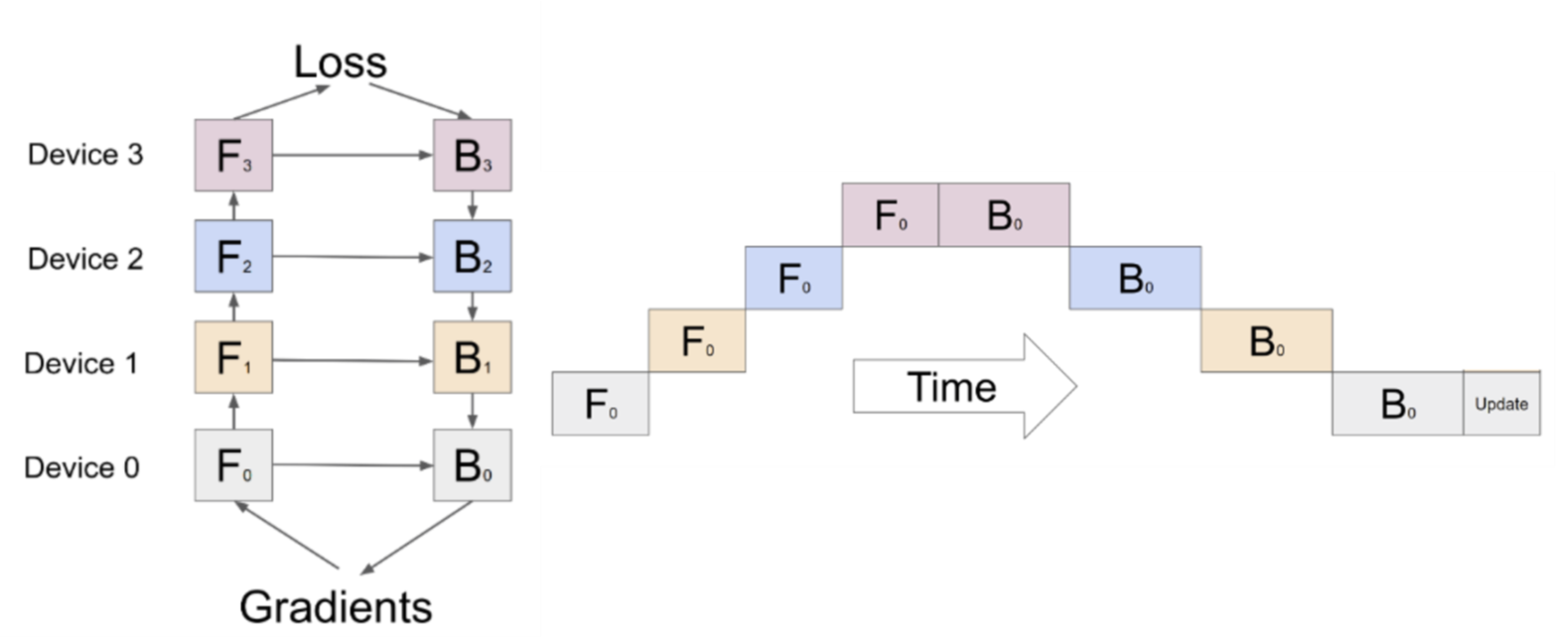
\includegraphics[scale=0.4]{NormalPipeline}
  \caption{Naive multiple modules}
  \label{fig:multiplemodule}
\end{figure}
Due to complex dependencies between the sequential modules, simply splitting the model will cause excessive stall time, a.k.a. bubble time. As shown in Figure \ref{fig:multiplemodule}, if we split the model into 4 modules $m_0,m_1,m_2,m_3$, there will be sequential dependencies between the forward pass $F_0, F_1, F_2, F_3$ of modules $m_0,m_1,m_2,m_3$, and reverse dependencies between backward pass $B_3, B_2, B_1, B_0$. The dependencies between the forward pass and backward pass will force strict ordering between modules, introduce synchronizations at module boundaries, and cause significant idle time on 4 devices. \par
 \begin{figure}[htbp]
  \centering
  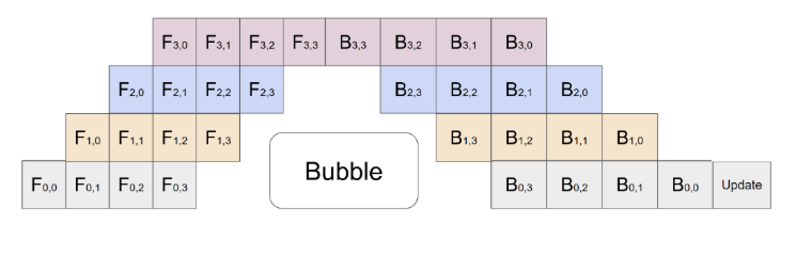
\includegraphics[scale=0.45]{stackedpipeline}
  \caption{Pipeline Parallelism}
  \label{fig:stackedpipeline}
\end{figure}
\subsection{Stacked Pipeline Parallelism}
Our approach is similar to GPipe\cite{huang2019gpipe}. We split a batch into multiple micro-batches and sequentially run the forward and backward pass of multiple micro-batches. We call this Stacked Pipeline Parallelism because different micro-batches are stacked. Dependencies now only exist between the forward and backward pass of the same micro-batch. Different modules of different micro-batches could run in parallel as shown in Figure \ref{fig:stackedpipeline}. Stacked Pipeline Parallelism allows users to fully utilize distributed devices by minimizing stall time caused by cross-module dependencies. \par
Stacked Pipeline Parallelism will insert blocking send/recv operations at the module boundaries to maintain necessary data dependencies. The gradient of multiple micro-batches will be accumulated and used to update weight synchronously for the entire mini-batch. Stacked Pipeline Parallelism can easily scale to a large number of devices while maintaining ideal utilization of resources.\par
Stacked Pipeline Parallelism will introduce little communication overhead because it will only transfer data at the module boundaries. This feature of Stacked Pipeline Parallelism makes it suitable both for systems with high-speed interconnections and weakly connected systems. \par
Throughout the rest of this paper, the term Pipeline Parallelism refers to Stacked Pipeline Parallelism.
 \subsection{Pipeline Parallelism in AIRCoP}
 Pipeline Parallelism in AIRCoP is done through module annotation systems. The annotation consists of an integer representing the number of micro-batches, a.k.a. pipelines.
 Users can split the model into several modules and annotate them to achieve Pipeline Parallelism. The resulting training loop is different from naively partitioned modules.
 \begin{align*}
  \textbf{ModuleAnnotation}: \qquad \qquad& \\
  a \in PipeAnno  := \mathcal{K} (\epsilon : \mathcal{N})\qquad \qquad&
\end{align*}
For $\epsilon$ pipelines, the target program will have a top-level training loop for iterating mini-batches. Inside each mini-batch iteration, a training loop of size $\epsilon$ is used to iterate the forward pass of the $\epsilon$ micro-batches, another training loop of size $\epsilon$ is used to iterate the backward pass of the $\epsilon$ micro-batches. The gradient will be accumulated inside each backward pass of micro-batches. The weight will be updated based on gradient descent for the entire mini-batch when the backward pass training loop ends.
 \section{Formal description of Pipeline Parallelism Transformation}\label{formalpipe}
%\begin{align*}
%  \textbf{ModuleAnnotation}:& \\
%  a \in PipeAnno & := \mathcal{K} (\epsilon : \mathcal{N}) \\
%  \textbf{Model}:&\\
%   s\_model \in Model&:= \quad List[Module \textbf{ by } PipeAnno] \\
%   \textbf{Transformation}:&\\
%   Transform&:Model \rightarrow Model \\
%   Transform (module::modulelist)&\triangleq Transform(module)::Transform(modulelist)\\
%   Transform (module \in Module)&\triangleq Collection(module)(\emptyset,\emptyset,\emptyset)\\
%   \textbf{Collection Phase}:&\\
%   Collection: Module \rightarrow List[Var \times Operation]& \rightarrow List[Var \times Operation] \rightarrow List[Var \times operation] \rightarrow Module \\
%   Collection(\textbf{let } xs = &Weight([], ots) \textbf{ in } module)(E_w,E_f,E_b)\triangleq \\
%   Collection&(module)(E_w :: (xs, Weight([], ots), E_f,E_b) \\
%   Collection(\textbf{let } xs = &Input([], ots) \textbf{ in } module)(E_w,E_f,E_b)\triangleq \\
%   Collection&(module)(E_w, E_f :: (xs, Input([], ots)),E_b) \\
%   Collection(\textbf{let } xs = &ml\_op(ins, ots) \textbf{ in } module)(E_w,E_f,E_b)\triangleq \\
%   Collection(module)(E_w, &E_f :: (xs, ml\_op(ins, ots)),(ins^\prime, ml\_op^\prime(ins::xs::xs^\prime, ins.tt))::E_b) \\
%   Collection(xs)&(E_w,E_f,E_b) \quad if \text{ (xs is not used in subsequent module)}\triangleq\\
%   Generation(E_w, &E_f,(xs^\prime, One([], xs.tt))::E_b) \\
%   Collection(xs)&(E_w,E_f,E_b) \quad if \text{ (xs is used in subsequent module)}\triangleq\\
%   Generation(E_w, &E_f::([], Send([xs],xs.tt)),(xs^\prime, Recv([], xs.tt))::E_b) \\
%   \textbf{Generation Phase}:&\\
%\end{align*}
Transformation for Pipeline Parallelism has 2 stages: \textbf{Collection Phase} and \textbf{Generation Phase}. The Collection Phase collects the necessary information like forward/backward operation. The Generation Phase uses the collected information and the module annotation to generate the training loop.\par
\paragraph{Collection Phase}
During Collection Phase we need to collect the weight operations $E_w$, forward operations $E_f$ and backward operations $E_b$. For Pipeline Parallelism, we will add send/recv into $E_f$ and $E_b$ to maintain the data dependencies between modules. $xs^w$, $xs^f$, $xs^b$ are the corresponding variables of $E_w$, $E_f$, $E_b$. The lift variables are calculated as: $$xs^l = Defined(E_f) \bigcap Used(E_b)$$The lifted variables $xs^l$ are the variables defined in the forward pass and used in the backward pass. We need to lift $xs^l$ into the outer scope and keep multiple versions of those variables for different micro-batches because we are generating different loops for forward pass and backward pass of micro-batches.\par
\paragraph{Generation Phase}
The formal description of the Generation Phase is as follows:
\begin{align*}
  \textbf{Generation Phase}: \qquad \qquad& \\
  G(E_w,E_f,E_b, xs^w,xs^f,xs^b,xs^l,\alpha:\mathcal{K} (\epsilon))& \triangleq \\
  G_w(E_w)G_l(xs^l)(loop \text{  } i=[0\dots n/\epsilon] &\textbf{ in}\\
  loop \text{  }j=[0\dots \epsilon]\text{ }G_f(E_f, xs^l) \textbf{ then}&\\
  loop \text{  }j=[0\dots \epsilon]\text{ }G_b(E_b, xs^f) \textbf{ then}&\\
  G_o(xs^w) \textbf{ then } xs^w\quad \qquad \qquad&
\end{align*}
\begin{align*}
  G_w&((xs, Weight([], out\_type))::E_w)\triangleq\\
  &\textbf{let } xs=Weight([], out\_type) \textbf{ in}\\
  &\textbf{let } xs^\prime=Zero([], out\_type) \textbf{ in}\\
  &\textbf{let } xs^m=Zero([], out\_type) \textbf{ in}\\
  &G_w(E_w)\\
  G_l&(xs::xs^l)\triangleq\\
  &\textbf{let } xs^\epsilon=Zero^\epsilon([], xs.type) \textbf{ in}\\
  &G_l(xs^l)\\
  G_f&((xs, op([input], out\_type))::E_f, xs^l)\triangleq\\
  &\textbf{let } xs=op([input], out\_type) \textbf{ in}\\
  &G_f(E^f, xs^l)\\
  G_f&(\emptyset, xs::xs^l)\triangleq\\
  &\textbf{let } \phi=Assign([xs, xs^\epsilon], xs.type) \textbf{ in}\\
  &G_f(\emptyset, xs^l)\\
  G_b&(E_b, xs::xs^f)\triangleq\\
  &\textbf{let } xs^\prime=Zero([], out\_type) \textbf{ in}\\
  &G_b(E^b, xs^f)\\
  G_b&((xs^\prime, op^\prime([input], out\_type))::E_b, \emptyset)\triangleq\\
  &\textbf{let } t=op^\prime_l([input], out\_type) \textbf{ in}\\
  &\textbf{let } \phi=Accumulate([t, xs^\prime], out\_type) \textbf{ in}\\
  &G_b(E^b, \emptyset)\\
  G_o&(xs::xs^w)\triangleq\\
  &\textbf{let } \phi=Optimize([xs,xs^\prime,xs^m], xs.type) \textbf{ in}\\
  &G_o(xs^w)\\
  \\
  op_l&([input],out\_type) \triangleq op([input^\epsilon], out\_type)
\end{align*}
where $op_l$ means that the operation will read from the versioned lift variable instead of the original variable. $xs^\epsilon = Zero^\epsilon$ will generates an array of $\epsilon$ versions of the variable $xs$.\par
$G_w$ generates the weight and their gradient and momentum, $G_l$ generate an array of lift nodes for different micro-batches, $G_f$ generates forward pass and write the correct value to the versioned lift variables, $G_b$ generates the backward pass and read from the versioned lift variable, $G_o$ generates the optimization pass. All the mutation operations (Assign/Accumulate/Optimize) are automatically generated in the Generation Phase because our source language does not allow mutation. We only need to write the versioned lift node at the end of the forward pass, and the Generation phase can generate the correct training loop.
\section{Implementation} \label{implementation}
We implement AIRCoP and Stacked Pipeline Parallelism in LMS compiler framework\cite{rompf2010lightweight}, and generate CUDA\cite{sanders2010cuda} code with MPI\cite{gropp1999using}/NCCL for communication as the target executable program.\par
\subsection{Integration into LMS}
LMS (Lightweight Modular Staging) is a library-based staging compiler that distinguishes stages solely based on Type information. LMS is beneficial for developing DSL through overloading. It has a typed frontend making the code generation safe. LMS offers lifted (next-stage) versions of regular operators and standard control-flow statements, making symbolic code generation easy and convenient. AIRCoP is simply a tensor computation DSL embedded inside LMS framework.\par
We embedded the formal syntax of AIRCoP inside the IR of LMS. LMS has ANF\cite{flanagan1993essence} form sea of Nodes\cite{click1995simple} IR. It also has an effect system to handle side effects and dependencies introduced by effects. LMS can perform Dead Code Elimination and Common Subexpression Elimination; therefore is sufficient for implementing our tensor computation graph transformation. LMS IR is customizable and offers users the flexibility to define their operation while maintaining the data and effect dependencies. We use custom IR nodes to represent Input/Weight Tensor and Machine learning Operations and use the effect system to represent their dependencies. The Module can be simply represented by a Node with a block that contains all of its operations. \par
The typed frontend source language of AIRCoP only contains the sequential forward computation of the model and annotations. The source language does not mutate tensors. We use overloading of the typed frontend objects and reflection to generate the corresponding IR of the source program. We put the explicit TensorType and Annotations into the RHS of the IR to make it persistent and used in later transformation. \par
\subsection{Training loop transformation For Pipeline Parallelism}
We use the transformation pass of LMS to transform the IR and simulate the tensor graph transformation to generate the correct training loop. We first perform DimName pass to merge the equivalent dimension of different tensors, e.g., if matrix multiplication happens between matrixes of dimension $[m, n]$ and dimension $[j,k]$, then dimension $n$ and dimension $j$ can be merged.  Annotations of tensors and operations represent which dimension to partition, so we must update those annotations. \par
The next pass DistributeTensorAIRCoP is the core pass to implement training loop transformation. This pass has 2 phases \textbf{Collection Phase} and \textbf{Generation Phase}.\par
\paragraph{Collection Phase}
The Collection Phase collects the forward operations, the weight nodes, and the corresponding backward operation of each node. The backward operation is collected in reverse order to maintain the correct semantic of differentiation. We collect backward operations as closures because the backward pass should be generated after the forward pass. The Collection Phase will also collect paired send/recv operations at the boundaries of different modules to maintain the correct data dependencies. We implement the Collection Phase by defining a function aircopCollect for each IR Node to collect the corresponding information. After the Collection Phase, we have obtained the necessary information to perform automatic differentiation, i.e., AD. We also need to collect lifted tensors to generate the correct training loop. As we mentioned before, the forward pass and backward pass of micro-batches are iterated in different loops to achieve Pipeline Parallelism. The tensors allocated in the forward pass and used in the backward pass will trigger an error because forward and backward passes are now in different scopes. These tensors are called lifted tensors. We have to lift them into the outer scope and maintain multiple versions of them as an array of tensors. Micro-batches' forward and backward passes will use different versions of the lifted tensors. After collecting the lifted tensors, the Collection Phase is finished.\par
\paragraph{Generation Phase}
The Generation Phase generates the correct training loop based on the collected information. It will first generate the top-level training loop of mini-batches for each module. Inside the body of the top-level loop, as we mentioned in Section \ref{formalpipe}, it will generate the forward training loop and backward training loop for micro-batches based on Module Annotations and use the collected backward operations to realize automatic differentiation. Inside both the forward and backward pass, the read and write to the lifted tensors will be transformed into read/write to the versioned tensor array. The weight gradient will be accumulated in the backward pass and optimized at the end of the entire mini-batch.\par
\subsection{Spatial Partition Pass}
The next pass will perform the Spatial Partition transformation. This part is of previous work, so we will not dig further into this pass. The main purpose of this pass is to partition the tensors and operations based on annotations and add the corresponding tensor communication between operations for synchronization, e.g., AllReduce for MatrixMultiplication and Convolution.\par
\subsection{MPI/NCCL Pass}
The final pass generates the corresponding MPI/NCCL instructions for inter-device communications. NCCL (NVIDIA Collective Communications Library) is the communication library designed by NVIDIA for efficient collective and point-to-point communication among multiple GPU and multiple Nodes. Our target program is CUDA code with MPI/NCCL for communication. We use MPI to set up the environment and the NCCL communicator. We will create 2 NCCL communicators, one global communicator for cross-module communication (NCCLSend/Recv) and one local communicator for collective tensor communication (NCCLAllReduce) inside modules. We also need to handle tensor communication between modules if they have different Spatial partitions, which can be implemented by gather and scatter. We use cuBLAS and cuDNN for matrix computation and convolution networks.\par
We statically allocate GPU memory before the training loop and avoid time-exhausting cudaMalloc/cudaFree inside the loop to optimize memory management. We currently use code-motion techniques to lift the cudaMalloc out of the training loop and pre-allocate the memory to optimize memory management. This approach could significantly improve performance because cudaMalloc/Free often occupies excessive time.\par
Our generated CUDA code can efficiently represent the correct training loop of machine learning models with Spatial Partition and Pipeline Parallelism.
 \section{Evaluation}\label{evaluation}
 This section shows the evaluation benchmarks of various forms of parallel training by running our generated CUDA code on 4 GeForce TITAN XP GPUs on server cuda.cs.purdue.edu. The server is a single GPU cluster with a high-speed inter-GPU connection. The ideal network topology for Pipeline Parallelism is an extensive training system consisting of several Nodes, but we currently could not run the evaluation under that scenario due to limited hardware resources and time. The purpose of this benchmark is to validate our graph transformation and gain a deeper insight into the choice of different parallelism strategies.\par
 We perform our test on a 12 layer convolution network for 40 iterations with different parallelism settings:
 \begin{itemize}
   \item Data Parallelism running on 2 GPUs
   \item Data Parallelism running on 4 GPUs
   \item Mixed Parallelism running on 4 GPUs --- Naively partitioned into 2 modules with each module running in Data Parallelism on 2 GPUs
   \item Mixed Parallelism running on 4 GPUs --- 2 modules in Stacked Pipeline Parallelism (4 pipelines) with each module running in Data Parallelism on 2 GPUs
   \item Mixed Parallelism running on 4 GPUs --- 2 modules in Stacked Pipeline Parallelism (8 pipelines) with each module running in Data Parallelism on 2 GPUs
 \end{itemize}
 \begin{figure}[htbp]
  \centering
  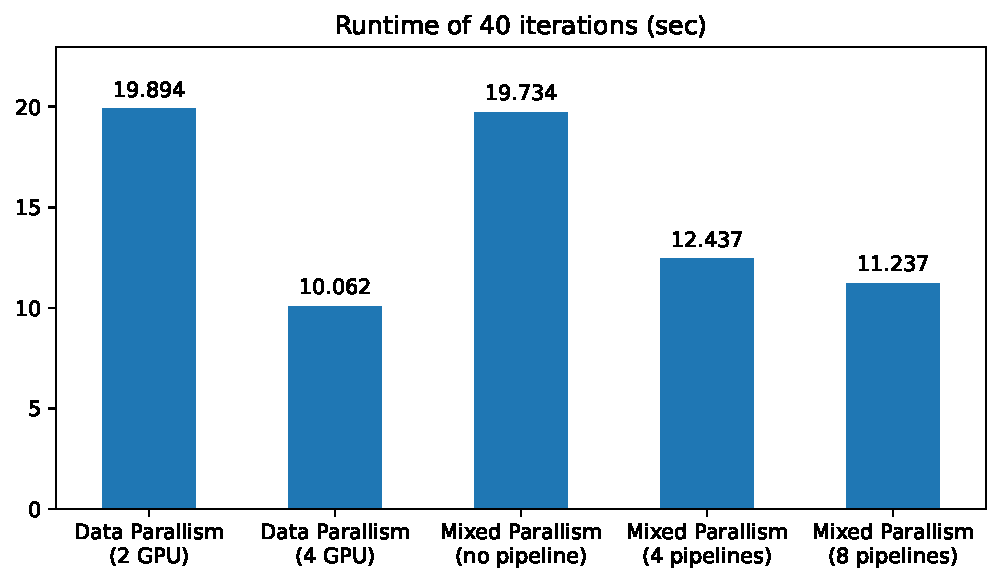
\includegraphics[scale=0.5]{pipelineparallelruntime.pdf}
  \caption{Data Parallelism vs Pipeline Parallelism}
  \label{fig:runtime}
\end{figure}
\begin{figure}[htbp]
  \centering
  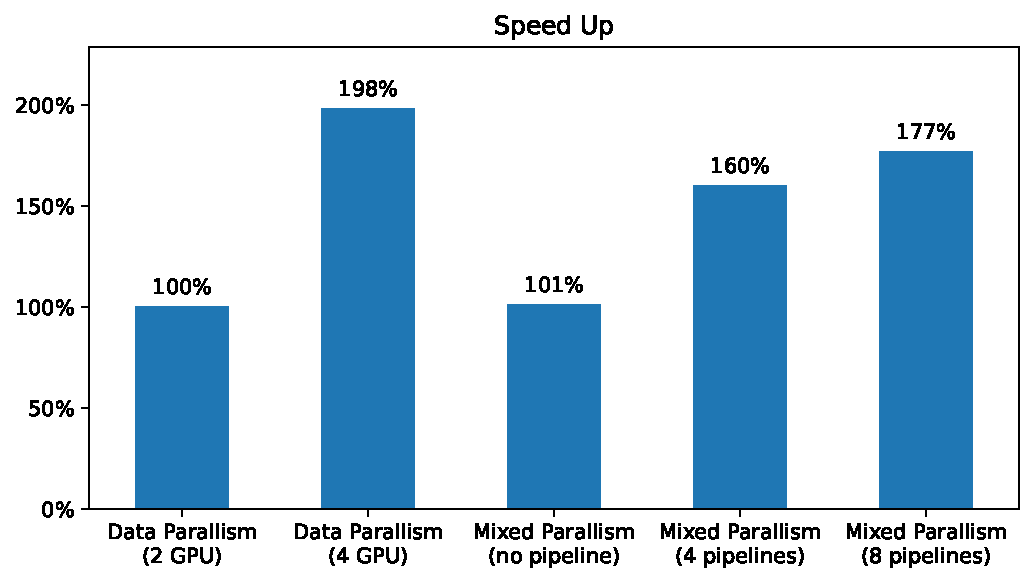
\includegraphics[scale=0.5]{pipelineparallelspeedup.pdf}
  \caption{Data Parallelism vs Pipeline Parallelism}
  \label{fig:speedup}
\end{figure}
The running time of 5 settings is shown in Figure \ref{fig:runtime}, the corresponding speedup is shown in Figure \ref{fig:speedup}. It can be observed that simply dividing a model into 2 modules will not cause any speed up due to the low device usage caused by the cross-module dependencies. The device will idle while waiting for data to arrive. We can notice that using Pipeline Parallelism with 4 pipelines rather than naive module partition on 2 modules will cause a speedup of 1.6x. Moreover, we can further accelerate the training loop by increasing the pipeline number, i.e., micro-batch number, to 8 and reach a speedup of 1.77x. However, increasing the pipeline number will cause the memory usage to surge due to versioned tensors.\par
The speedup achieved is significant and is very close to the theoretical limit. No matter how many pipelines we choose, some bubble time will still exist because the different modules of the same micro-batch will still have dependencies between them. For 2 modules, the theoretical speedup limit is $\frac{2n}{n+1}$ where $n$ is the pipeline number, which is about the same as our evaluation result.\par
However, we find that 2 modules on Stacked Pipeline Parallelism with each module running at Data Parallelism on 2 GPUs, i.e., Mixed Parallelism, still perform a little worse than Data Parallelism on 4 GPUs. This result is anticipated because we perform our evaluation on a single GPU cluster with very high-speed inter-GPU connections, which makes the frequent tensor communication (ALLReduce) overhead introduced by Data Parallelism negligible. However, the cross-module dependencies for micro-batch will still cause some bubble time. As we mentioned before, the ideal network topologies for Pipeline Parallelism are an extensive training system consisting of multiple GPU clusters connected through the network. Then we can use Data Parallelism inside each cluster and Pipeline Parallelism among clusters. We currently could not perform evaluation under this ideal scenario due to limited time and hardware resources, but we could deduce that Pipeline Parallelism mixed with Data Parallelism will perform much better than only using Data Parallelism under this scenario because Pipeline Parallelism could significantly reduce the communication overhead by restricting the inter-cluster communication to only happen at module boundaries.\par
 The evaluation shows that our framework is flexible, and the user could switch to different combinations of Parallelism settings to reduce the total communication overhead and achieve optimal performance. It also demonstrates that our framework can unify both Spatial Partition and Pipeline Parallelism, validates the correctness of our training loop transformation, and offers a deeper insight into how to choose between different parallel training settings.
 \section{Conclusion} \label{conclusion}
We implement Pipeline Parallelism for AIRCoP, make it a machine learning framework that can integrate different parallelism strategies, and offer user flexibility to fully explore different combinations of parallel training strategies under different hardware scenarios and gain a deeper insight into parallel training.
\bibliographystyle{acm}
\bibliography{paper}
\end{document}
\endinput
